\documentclass[tikz,border=3pt]{standalone}
\usepackage[utf8]{inputenc}
\usepackage[T1]{fontenc}
\usepackage{lmodern}
\renewcommand{\familydefault}{\sfdefault}
\usepackage{sansmath}\sansmath
\usepackage{chemfig}
\usepackage{pgfplots}\pgfplotsset{compat=1.18,/pgf/number format/use comma,/pgf/number format/1000 sep={.}}
\usetikzlibrary{arrows.meta,calc,positioning,decorations.pathmorphing,patterns}
% paleta del sitio
\definecolor{nar}{HTML}{E8680C}\definecolor{narc}{HTML}{FFB35C}\definecolor{hielo}{HTML}{FFF3E8}
\definecolor{tinta}{HTML}{1D1D1F}\definecolor{gris}{HTML}{6E6E73}\definecolor{lila}{HTML}{7C5CF0}
\definecolor{azul}{HTML}{2F6FD6}\definecolor{menta}{HTML}{17A673}\definecolor{coral}{HTML}{E8342A}
\begin{document}
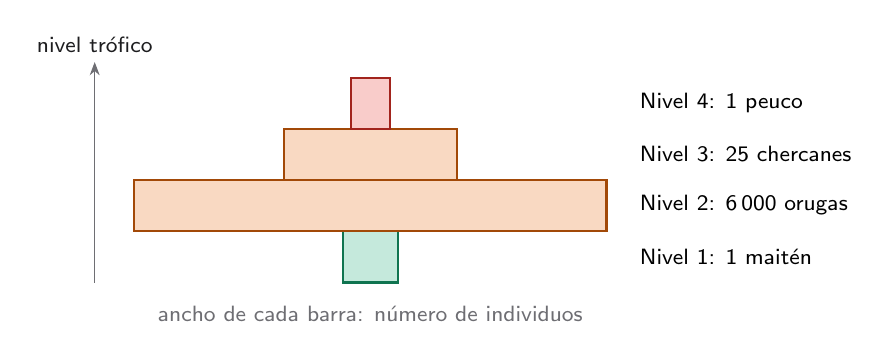
\begin{tikzpicture}[font=\footnotesize]
\tikzset{bar/.style={draw=#1!70!black,fill=#1!25,thick}}
\draw[bar=menta] (-0.35,0) rectangle (0.35,0.65);
\draw[bar=nar] (-3.0,0.65) rectangle (3.0,1.3);
\draw[bar=nar] (-1.1,1.3) rectangle (1.1,1.95);
\draw[bar=coral] (-0.25,1.95) rectangle (0.25,2.6);
\node[anchor=west] at (3.3,0.33) {Nivel 1: 1 maitén};
\node[anchor=west] at (3.3,0.98) {Nivel 2: 6\,000 orugas};
\node[anchor=west] at (3.3,1.63) {Nivel 3: 25 chercanes};
\node[anchor=west] at (3.3,2.28) {Nivel 4: 1 peuco};
\draw[gris,->,>={Stealth}] (-3.5,0) -- (-3.5,2.8) node[anchor=south,text=tinta] {nivel trófico};
\node[text=gris] at (0,-0.4) {ancho de cada barra: número de individuos};
\end{tikzpicture}
\end{document}
